\documentclass[11pt]{article}

\usepackage{tikz}
\usepackage{amsmath}
\usetikzlibrary{calc, shapes, backgrounds, arrows}

\author{Parham Alvani}
\title{Computer Architecture Homework 1}
\begin{document}
\begin{titlepage}
\begin{center}
\emph{In The Name of God}
\end{center}
\maketitle
\begin{center}
powered by \LaTeX
\end{center}
\end{titlepage}
\tableofcontents
\newpage
\section{Problem 1}

% Define block styles
\tikzstyle{decision} = [diamond, draw, fill=blue!20,
	text width=4.5em, text badly centered, node distance=3cm, inner sep=0pt]
\tikzstyle{block} = [rectangle, draw, fill=blue!20,
	text width=5em, text centered, rounded corners, minimum height=4em]
\tikzstyle{line} = [draw, -latex']
\tikzstyle{cloud} = [draw, ellipse,fill=red!20, node distance=3cm,
	minimum height=2em]

\begin{tikzpicture}[node distance = 2cm, auto]
	\node [block] (A) {A};
	\node [decision, right of=A] (inputA) {En};
	\node [block, right of=inputA, node distance=3cm] (B) {B};
	\node [decision, below of=B] (inputB) {En};
	\node [block, right of=inputB, node distance=3cm] (C) {C};
	\node [decision, below of=C] (inputC) {En};
	\node [block, right of=inputC, node distance=3cm] (D) {D};
	\node [decision, below of=D] (inputD) {En};
	\node [cloud, left of=inputD] (outputD) {X};

	\path [line] (A) -- (inputA);
	\path [line] (inputA) -- node [near start] {no} (A);
	\path [line] (inputA) -- node [near start] {yes} (B);
	\path [line] (B) -- (inputB);
	\path [line] (inputB) -- node [near start] {no} (B);
	\path [line] (inputB) -- node [near start] {yes} (C);
	\path [line] (C) -- (inputC);
	\path [line] (inputC) -- node [near start] {no} (C);
	\path [line] (inputC) -- node [near start] {yes} (D);
	\path [line] (D) -- (inputD);
	\path [line] (inputD) -- node [near start] {no} (D);
	\path [line] (inputD) -- node [near start] {yes} (outputD);
	\path [line] (outputD) -| (A);
\end{tikzpicture}

\section{Problem 2}
\paragraph{1}
\paragraph{2}
According to following diagram :

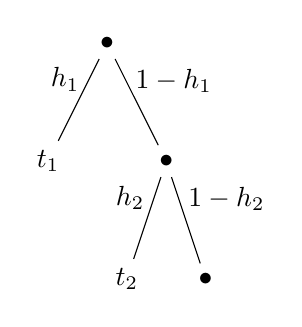
\begin{tikzpicture}[level 2/.style={sibling distance=10mm}]
	\node (START) {$\bullet$}
		child { node (T1) {$t_1$}}
		child { node (@T1) {$\bullet$}
			child {node (T2) {$t_2$}}
		child {node (@T2) {$\bullet$}}
		};
	\begin{scope}[nodes = {draw = none}]
		\path (START) -- (T1)  node [near start, left]  {$h_1$};
    		\path (START) -- (@T1) node [near start, right] {$1 - h_1$};
		\path (@T1)   -- (T2)  node [near start, left]  {$h_2$};
		\path (@T1)   -- (@T2) node [near start, right] {$1 - h_2$};
	\end{scope}
\end{tikzpicture}

\begin{itemize}
\item
	Average Memory Access Time, the exact formula
	\begin{equation}
		\label{eq:AMAT-e}
		t_1 + (1 - h_1) * [t_2 + (1 - h_2) * [\ldots]]
	\end{equation}	
\item
	Average Memory Access Time, an approximate formula
	\begin{equation}
		\label{eq:AMAT-a}
		h_1 * t_1 + (1 - h_1) [h_2 * t_2 + (1 - h_2) * [\ldots]]
	\end{equation}
\end{itemize}
\paragraph{3}
\paragraph{4}
\paragraph{5}
\section{Problem 3}
The following is the avrage memory access time equlation for
memory with 3 level:
\begin{equation}
	\label{eq:AMAT-3}
	\bar{T} = h_1 * t_1 + (1 - h_1) * h_2 * t_2 + (1 - h_1) * (1 - h_2) * h_3 * t_3
\end{equation}
Substituting $1ns$ for $t_1$, $0.9$ for $h_1$, $10ns$ for $t_2$, $0.5$ for $h_2$, $1000ns$ for $t_3$ and $1$ for $h_3$
in (\ref{eq:AMAT-3}) gives us:
\begin{align*}
	\bar{T} &= 0.9 * 1 + (1 - 0.9) * 0.5 * 10 + (1 - 0.9) * (1 - 0.5) * 1000\\
	&= 0.9 + 0.1 * 0.5 * 10 + 0.1 * 0.5 * 1000\\
	&= 0.9 + 0.5 * 10 + 0.5 * 1000\\
	&= 0.9 + 5 + 500.00\\
	&= 505.9ns
\end{align*}
\section{Problem 4}
The following is the avrage memory access time equlation for
memory with 4 level:
\begin{equation}
	\label{eq:AMAT-4}
	\bar{T} = h_1 * t_1 + (1 - h_1) * h_2 * t_2 + (1 - h_1) * (1 - h_2) * h_3 * t_3 + (1 - h_1) * (1 - h_2) * (1 - h_3) * h_4 * t_4
\end{equation}
Substituting $1ns$ for $t_1$, $0.9$ for $h_1$, $10ns$ for $t_2$, $0.5$ for $h_2$, $8s$ for $t_3$, $0.63$ for $h_3$,$1000ns$ for $t_4$, $1$ for $h_3$,
in (\ref{eq:AMAT-4}) gives us:
\begin{align*}
	\bar{T} &= 0.9 * 1 + (1 - 0.9) * 0.5 * 10 + (1 - 0.9) * (1 - 0.5) * 0.63 * 8 + \\
	&\qquad \phantom{= 0.1 * 1 + (1 - 0.9)} (1 - 0.9) * (1 - 0.5) * (1 - 0.63) * 1000 \\
	&= 0.9 * 1 + 0.1 * 0.5 * 10 + 0.1 * 0.5 * 0.63 * 8 + 0.1 * 0.5 * 0.37 * 1000 \\
	&= 0.90 + 0.50 * 10 + 0.31 * 8 + 0.18 * 1000 \\
	&= 0.90 + 5.00 + 2.48 + 180.00 \\
	&= 188.38ns
\end{align*}
\section{Problem 5}
\paragraph{1}
Adrress bits $= 14$ bits, \qquad Length $= 2$ bytes, \qquad Width $= 2^{14}$ words, \qquad The smallest unit available $= 16$ bits.
\paragraph{2}
Adrress bits $= 15$ bits, \qquad Length $= 2$ bytes, \qquad Width $= 2^{15}$ words, \qquad The smallest unit available $= 16$ bits.
\paragraph{3}
Adrress bits $= 15$ bits, \qquad Length $= 1$ bytes, \qquad Width $= 2^{15}$ words, \qquad The smallest unit available $= 8$ bits.
\paragraph{4}
Adrress bits $= 13$ bits, \qquad Length $= 4$ bytes, \qquad Width $= 2^{13}$ words, \qquad The smallest unit available $= 32$ bits.
\end{document}
